\chapter{\textbf{Methodology}} \label{cap:methodology}

The traditional approach in terms of economic sentiment is the construction of sentiment indices through surveys \cite[p.4]{shapiro2020measuring} -- ``Usually, these surveys are monthly, with interviews and even verification of the interviewees' personal finances'' \cite[p. 5]{shapiro2020measuring}. The idea of this work is to obtain a sentiment index through sentiment analysis and Natural Language Processing techniques.

\section{Natural Language Processing}

According to \cite{liddy2001natural}, Natural Language Processing (NLP) is a computational approach to textual analysis that is based on both a set of theories and a set of technologies. In other words, by the formal definition, ``Natural Language Processing is a theoretically motivated range of computational techniques for analyzing and representing naturally occurring texts at one or more levels of linguistic analysis for the purpose of achieving human-like language processing for a range of tasks or applications'' \cite[p. 2]{liddy2001natural}. The purpose of this tool is, therefore, ``to accomplish human-like language processing''. In general, the classification of a text, phrase, or even word is given categorically according to its positivity (positive, negative, neutral), or through valence scores, from 1 to 5. ``The sentiment of text is a measure of the speaker's tone, attitude, or evaluation of a topic, independent of the topic's own sentiment orientation (e.g., a horror movie can be `delightful')'' \cite[p. 5]{shapiro2020measuring}.\\

The present work will use lexical-based NLP techniques. ``At this level, humans, as well as NLP systems, interpret the meaning of individual words. Several types of processing contribute to word-level understanding – the first of these being assignment of a single part-of-speech tag to each word. In this processing, words that can function as more than one part-of-speech are assigned the most probable part-of-speech tag based on the context in which they occur'' \cite[p.7]{liddy2001natural}. Still, ``Additionally at the lexical level, those words that have only one possible sense or meaning can be replaced by a semantic representation of that meaning. The nature of the representation varies according to the semantic theory utilized in the NLP system. The following representation of the meaning of the word launch is in the form of logical predicates. As can be observed, a single lexical unit is decomposed into its more basic properties. Given that there is a set of semantic primitives used across all words, these simplified lexical representations make it possible to unify meaning across words and to produce complex interpretations, much the same as humans do'' \cite[p.7]{liddy2001natural}.\\

\section{Sentiment Analysis and Lexicons}

In the scope of sentiment analysis, it is necessary to use a dictionary of sentiments to detect polarities of sentiments and positive/negative scores. From the scores and polarities, it is possible to obtain a sentiment index that generates a possible correlation with the macroeconomic scenario. Basically, a sentiment dictionary works by indicating a specific punctuation for each word, taking into account punctuation and connectives. That is, depending on how a sentence or sentence is written, its polarity (score) varies.\\


\subsection{Sentiment Lexicons} \label{sec:lexicons}
One of the most adopted and valuable resources for sentiment analysis is the use of sentiment lexicons \cite[]{ahire2014survey, nusko2016building, cambria2013new, kaity2020sentiment}. A sentiment lexicon is a collection of words (sometimes referred to as polar or opinion words) linked to their sentiment orientation, that is, positive or negative \cite[]{kaity2020sentiment, medhat2014sentiment}.

\subsection{Valence-based Lexicons and the VADER – Valence Aware Dictionary for sEntiment Reasoning}

A valence-based lexicon can be justified by the need that when analyzing a text or phrase the expected results can be not only binary (positive and negative), but determined by the ``intensity'' of each word or phrase \cite[] {hutto2014vader}. When considering a valence-based lexicon, polarity is the main focus in determining the scores of \cite[]{cambria2012senticnet} words and texts. The authors develop a valence-based lexicon so that texts and words have values such that the $score_i$ (with $i$ being a word, text or even phrase) ranges from $-1$ to $1$, so that $ score_i \subset (-1, 1) \quad \forall \quad score_i \in \mathbb{R}$.\\

Even though \cite{cambria2020senticnet} is a valence-based lexicon implemented in Python, compared to other valence-based lexicons \cite[]{hutto2014vader} gives inferior results to other valence-based lexicon.\\


%\subsection{VADER – Valence Aware Dictionary for sEntiment Reasoning} %\label{subsec:vader}

Another lexicon, VADER, or Valence Aware Dictionary for sEntiment Reasoning is a lexicon initially created as a parsimonious lexicon for social media text. However, it has been used in general cases of textual sentiment analysis given it's benchmarks compared to other lexicons or even machine learning oriented techniques ``relying on Naive Bayes, Maximum Entropy, and Support Vector Machine (SVM) algorithms'' \citep[p.216]{hutto2014vader}. Differently of most part of lexicons, VADER was created taking into account a combination of qualitative and quantitative methods to empirically validates and produces a \textit{golden-standard} sentiment lexicon \cite{hutto2014vader}.\\

Due to the fact that VADER is an open-source lexicon, it is relatively simple to modify -- even if it is not what was done in this work, it would be possible, if necessary, merging VADER with some other lexicons, with the objective of creating a more complex and dense lexicon focused on economic science and finance. This lexicon has about 7520 words and textual forms with a classified score compound which after normalized varies from -1 to 1 such that:
\begin{align} \label{eq:vaadercoumpond}
    score_ = \begin{cases}
                positive\quad if \quad compound > 0.05\\
                neutral\quad if \quad 0.05 \geq compound \geq -0.05\\
                negative\quad if \quad compound < 0.05
              \end{cases} \qquad \forall\quad compound \in (-1, 1)
\end{align}

The positive, neutral and negative scores are ratios for each category that the text or expression fells on: 
\begin{quote}
    ``These are the most useful metrics if you want to analyze the context \& presentation of how sentiment is conveyed or embedded in rhetoric for a given sentence. For example, different writing styles may embed strongly positive or negative sentiment within varying proportions of neutral text -- i.e., some writing styles may reflect a penchant for strongly flavored rhetoric, whereas other styles may use a great deal of neutral text while still conveying a similar overall (compound) sentiment. As another example: researchers analyzing information presentation in journalistic or editorical news might desire to establish whether the proportions of text (associated with a topic or named entity, for example) are balanced with similar amounts of positively and negatively framed text versus being "biased" towards one polarity or the other for the topic/entity'' \cite{vadergit}.
\end{quote}

Even when VADER excels when in social media, it's scores benchmarks when considered newspaper editorials are higher above the other lexicons or machine learning techniques (Table \ref{tab:vaderscore}) -- ``Surprisingly, when we further inspect the classification accuracy, we see that VADER (F1 = 0.96) actually even outperforms individual human raters (F1 = 0.84) at correctly classifying the sentiment of tweets into positive, neutral, or negative classes'' \citep[p.216]{hutto2014vader}.

\begin{table}[!h]
\centering
\caption{VADER 3-class classification performance as compared to individual human raters and 7 established lexicon baselines}
\begin{tabular}{l|c|c|c|c}
\hline
\multicolumn{2}{l|}{Correlation to ground truth} & \multicolumn{3}{l}{Classification Accuracy Metrics}   \\ \cline{3-5} 
\multicolumn{2}{l|}{(mean of 20 humans raters)}  & Overall Precision & Overall Recall & Overall F1 score \\ \hline
\multicolumn{5}{c}{NY Times Editorials (5,190 article snippets)}                                         \\ \hline
Ind. Humans                & 0.745               & 0.87              & 0.55           & 0.65             \\
VADER                      & 0.492               & 0.69              & 0.49           & 0.55             \\
Hu-Liu04                   & 0.487               & 0.70              & 0.45           & 0.52             \\
SCN                        & 0.252               & 0.62              & 0.47           & 0.38             \\
GI                         & 0.362               & 0.65              & 0.44           & 0.49             \\
SWN                        & 0.262               & 0.57              & 0.49           & 0.52             \\
LIWC                       & 0.220               & 0.66              & 0.17           & 0.21             \\
ANEW                       & 0.202               & 0.59              & 0.32           & 0.35             \\
WSD                        & 0.218               & 0.55              & 0.45           & 0.47             \\ \hline 
\end{tabular}
\caption*{Source: \citep[p. 223]{hutto2014vader}}
\label{tab:vaderscore}
\end{table}

\subsection{Polarity-based Lexicons and the Loughran-McDonald: LM-SA-2020} \label{subsec:polbas}

Polarity-based Lexicons are lexicons that allow you to automatically evaluate a text based on its polarity. These lexicons are ``a basic resource for analyzing the sentiments and opinions expressed in texts'' \cite[p.938]{san2016polarity}. When analyzing a text from the perspective of sentiment analysis, a polarity-based lexicon, words and phrases are commonly classified as positive, neutral and negative. If we take the example of the phrase ``Good people sometimes have bad days'', a polarity-based lexicon would possibly classify the word ``Good'' being a \textit{positive} word and the word ``bad'' would probably be classified as \textit{negative} -- the other words in the sentence would possibly be classified as ``neutral'' \cite[]{BCDG07}.\\

In terms of score classification, \cite{BCDG07} shows that in proportional and popular values a positive score can be presented as:
\begin{align*}
score = \frac{\text{number of positive words - number of negative words}}{\textit{number of positive words + number of negative words}}
\end{align*}

where \textit{number of positive words} would be the total number of positive words in a sentence or text and \textit{number of negative words} would be the total number of negative words in a sentence or text.\\

A possible barrier observed is in relation to the elaboration of a polarity-based lexicon and the way in which a lexicon is created \cite[]{stone1966general}. The vast majority of polarity-based lexicon is aimed at generic texts (without a specificity) -- when extracting sentiments from specific texts (such as economic and financial) a lexicon could present spurious results for not taking into account words that in the economic field can be considered positive or negative (the vast majority of lexicons do not include words and economic terms such as ``inflation'', ``recession'', or other such terms) \cite[]{loughran2011liability}.\\

\begin{table}[!h]
\caption{Examples of polarities in a polarity-based lexicon -- LM-SA-2020}
\adjustbox{max width=\textwidth}{
\begin{tabular}{ll|ll|ll|ll}
\hline
Word       & Polarity & Word        & Polarity & Word          & Polarity & Word        & Polarity \\ \hline
Abundance  & Positive & Abandon     & Negative & Inspirational & Positive & Defensive   & Negative \\
Abundant   & Positive & Abdicated   & Negative & Invented      & Positive & Dever       & Negative \\
Acclaimed  & Positive & Abdicates   & Negative & Inventor      & Positive & Deficit     & Negative \\
Accomplish & Positive & Aberrant    & Negative & Leadership    & Positive & Defraud     & Negative \\
Advances   & Positive & Aberrations & Negative & Leading       & Positive & Defunct     & Negative \\
Achieves   & Positive & Abrupt      & Negative & Lucrative     & Positive & Degradation & Negative \\ \hline
\end{tabular}
}
\caption*{Source: Words and polarities taken from \cite[]{lmdata}}
\label{tab:polarity}
\end{table}

Table \ref{tab:polarity} presents examples of a lexicon based on polarities. Note, however, that this lexicon was constructed based on economic terms and words, based on over 10,000 economic and financial articles \cite[p.1]{lmdata}.\\

In general, when a polarity-based lexicons is applied to a text, more advanced computational techniques are not necessary, except for an interactive algorithm that computes the polarity of the text \cite[]{BCDG07}.\\ 

The other lexicon used in this work is the LM-SA-2020 and was the same provided by \cite{loughran2011liability}. Fundamentally, the difference between this one is the composition: the authors developed a dictionary with the purpose of revising the traditional lexicons in which certain words are or are not considered positive or negative in the economic and financial sphere \citep[p. 35]{loughran2011liability}:

\begin{quote}
    ``The motivation for building the LM-SA-2020 word list was based on an experiment using the above-mentioned original lists to detect sentiment-carrying words in South African financial article headlines''\citep[p. 1]{lmdata}
\end{quote}

This lexicon uses 808 financial articles and only about 37\% of the headlines actually corresponded to the expected sentiments (either in terms of words or expressions) given the articles verified by the authors\citep{loughran2011liability}. In terms of benchmark, with adding economic words and removing others in terms of polarity, sentiment detection and prediction increased by about 29\% when added to NLTK's WordNet\footnote{\url{https://www.nltk.org/howto/wordnet.html}}.\\

The results obtained by the authors were based on an analysis of two samples of reference articles: first, the authors considered a sample of 10 thousand files related to ``firms subject to shareholder litigation under Rule 10b-5''\cite[p. 41]{loughran2011liability}. The other sample used by the authors considers \cite{doyle2007accruals}, between August 2002 and November 2005, companies disclosed at least one material deficiency in internal control \citep[p. 41]{loughran2011liability}. The authors estimated different models\footnote{In fact, 28 different Logit models were estimated. The economic variables used were ``The number of shares outstanding times the price of the stock as reported by CRSP on the day before the file date''\cite[p.63]{loughran2011liability}; ``Book-to-market (Derived from the Compustat and CRSP data items as specified in Fama and French (2001). The variable is based on the most recent Compustat data no more than 1 year before the file date. After eliminating observations with negative book-to-market, we winsorize the book-to-market variable at the 1\% level)''\cite[p.63]{loughran2011liability}; ``The volume of shares traded in days [−252, −6] prior to the file date divided by shares outstanding on the file date. At least 60 observations of daily volume must be available to be included in the sample''\cite[p.63]{loughran2011liability}; ``The prefile date Fama–French alpha based on a regression of their three-factor model using days [−252, −6]. At least 60 observations of daily returns must be available to be included in the sample''\cite[p.63]{loughran2011liability}; ``The percent of institutional ownership reported in the CDA/Spectrum database for the most recent quarter before the file date. The variable is considered missing for negative values and winsorized to 100\% on the positive side''\cite[p.63]{loughran2011liability}; ``The average volume of the 4-day event window [0, 3], where volume is standardized based on its mean and standard deviation from days [−65, −6]''\cite[p.63]{loughran2011liability}; ``The root-mean square error from a Fama–French three-factor model for days [6, 252], with a minimum of 60 daily observations''\cite[p.63]{loughran2011liability}; ``Standardized unexpected earnings for the quarterly earnings announced within 90 days after the 10-K file date. The actual earnings and the analyst forecast consensus (mean) are from I/B/E/S unadjusted files, which are used to avoid the rounding issue. The unexpected earnings are standardized with stock price''\cite[p.63]{loughran2011liability}; ``The standard deviation of analysts’ forecasts in the most recent period prior to the earnings announcement used to calculate SUE, scaled by the stock price at the end of the quarter''\cite[p.63]{loughran2011liability}; ''The monthly change in the mean of analysts’ forecasts, scaled by the stock price in the prior month''\cite[p.63]{loughran2011liability}; and a ``dummy variable set equal to one for firms whose shares are listed on the NASDAQ stock exchange, else zero''\citep[p.63]{loughran2011liability}} to reach the final conclusion that the lexicon accuracy increases with the addition or change of economic terms.\\

The lexicon created by the authors also allows for a more comprehensive classification in which, in addition to classifying certain words and terms as positive and negative, it also classifies them as ``uncertainty, litigious, strong modal, and weak modal words''\citep[p.62]{loughran2011liability}: 
\begin{quote}
    ``The paper finds evidence that some word lists are related to market reactions around the 10-K filing date, trading volume, unexpected earnings, and subsequent stock return volatility. [\dots] we show that financial researchers should be cautious when relying on word classification schemes derived outside the domain of business usage. Applying nonbusiness word lists to accounting and finance topics can lead to a high misclassification rate and spurious correlations''\citep[p.62]{loughran2011liability}
\end{quote}

\section{Modeling}

Two exercises are proposed, as previously mentioned. First, a case study will be carried out taking into account the inclusion of sentiment indices when considering economic models when utilizing Variable Selection Models criteria. For this, the LASSO, Adaptive LASSO and Elastic Net models are used.\\

The second case study refers to an Autoregressive Vector (VAR) -- impulse response functions are used to better understand the behavior of macroeconomic variables when a shock is given to one of the sentiment indices (VADER and LM- SA-2020).\\

\subsection{Variable Selection Models}
\label{sub:selection}

Variable selection models have as main objective the identification and statistically significant variables for a model. Unlike information criteria such as AIC \cite[]{akaike1974new} and BIC \cite[]{schwarz1978estimating}, the variable selection models used here are variations of the conventional LASSO model. That is, the selection of variables is done by forcing the coefficients related to each variable to 0 when not significant, so that when significant, the coefficients are greater than 0.\\

The first method of Variable Selection Models used in this first case study is the conventional LASSO. The LASSO estimator (least absolute shrinkage and selection operator) is a linear estimation method presented in 1996 in a paper entitled ``Regression Shrinkage and Selection via the LASSO'' \cite[]{tibshirani1996regression}. For regressions and generalized regressions, this estimator was proposed as a shrinkage and selection method.\\

Assuming a data set such that $(x^i, y_i)$ and $i = 1, 2, \dots , N$, and assuming $x^i = (x_{i1}, \dots, x_{ip})^T$ are the predictor variables and $y_i$ is the dependent variable. Also, since $\hat{\beta} = (\beta_1, \dots, \beta_p)^T$ the estimate LASSO $(\hat{\beta}^{LASSO})$ \cite[p. 268]{tibshirani1996regression} is given in its Lagrangian equivalent by:

\begin{align} \label{eq:LASSO}
    \hat{\beta}^{LASSO} = \frac{1}{2}(y - Xb)'(y - Xb) + \lambda\sum_{j=1}^p|b_j|
\end{align}
the penalty on $\sum_1 ^p |\beta_j|$ is called the L1 LASSO penalty \cite[p.68]{hastie2009elements} and this last constraint makes the solution nonlinear in $y_i$. The LASSO, however, ``does not focus on subsets but rather defines a continuous shrinking operation that can produce coefficients that are exactly 0''\cite[p.286]{tibshirani1996regression}. Thus, it can be seen that the greater $\lambda$, the greater the number of coefficients defined as 0.\\

Another estimator used in this case study as a variable selection model is the first variation of the LASSO presented here. The  Adaptive LASSO estimator was first described by \cite{zou2006adaptive} and, in contrast to LASSO, augments the penalty with a vector of weights. The adaptive LASSO estimator ($\hat{\beta}^{alasso}$), then, is given by:

\begin{align} \label{eq:lassoadaptive}
    \hat{\beta}^{alasso} = \frac{1}{2}(y - Xb)'(y - Xb) + \lambda\sum_{j=1}^p\hat{w}_j |b_j|
\end{align}

Where $\hat{w}_j$ is a vector of weights and can ``be given by $\hat{w}_j = \frac{1}{|b_{ols, j}|^\gamma}$, for some $ \gamma > 0$'' \cite[p. 115]{hoornweg2018science}.\\

The third variable selection model used here is the Elastic Net model \cite[]{zou2005regularization}. Despite the fact that there are more choices for other LASSO models, like the random LASSO \cite[]{wang2011random} and the group LASSO \cite[]{yuan2006model}, Elastic Net was used for being a well-known reference in the literature and for combining the L2 penalty\footnote{The L2 penalty is also known as Ridge regression \cite[p.2]{owen2007robust}.}:

\begin{align}\label{eq:elasticnet}
    \hat{\beta}^{enet} = \frac{1}{2}(y - Xb)'(y - Xb) + \lambda\sum_{j=1}^p\left(\frac{\alpha}{2}b_j ^2 + (1 - \alpha)|b_j|\right)
\end{align}
The formulation presented in (\ref{eq:elasticnet}) is the same formulation presented by \cite{hastie2009elements}. The Elastic Net model introduces a parameter $\alpha$ into the model so that when $\alpha = 0$ the model only incorporates the L1 LASSO penalty; and when $\alpha = 1$ the model only incorporates the L2 Ridge penalty; when $0 < \alpha < 1$ the Elastic Net model incorporates properties from both the LASSO model and the Ridge model.\\

The value of $\lambda$ in this case study is obtained by cross validation \footnote{see section \ref{sec:cv}} for the LASSO and Adaptive LASSO models, as well as the value of $\lambda$ and $\alpha $ for the Elastic Net model following the literature \cite[p. 136]{hoornweg2018science}.

\subsection{Vector Autoregression}

In order to consider a deeper analysis in terms of economic simulation, and taking into account the endogeneity characteristic, a Vector Autogression (VAR) model is estimated as a second case study. In mathematical terms, we can represent a VAR(1) in a matrix form, that is, a first-order Autoregressive Vector as follows:

\begin{align} \label{eq:var1}
    \begin{bmatrix}
    y_{1,t} \\
    y_{2,t}
    \end{bmatrix} = 
    \begin{bmatrix}
    \delta_1\\
    \delta_2
    \end{bmatrix} +
    \begin{bmatrix}
    \phi_{11} & \phi_{12} \\
    \phi_{21} & \phi_{22}
    \end{bmatrix}
    \begin{bmatrix}
    y_{1,t-1} \\
    y_{2,t-1}
    \end{bmatrix} +
    \begin{bmatrix}
    \varepsilon_{1,t} \\
    \varepsilon_{2,t}
    \end{bmatrix} 
\end{align}

Where $y_1$ and $y_2$ are endogenous variables and $\varepsilon_1$ and $\varepsilon_2$ are the error terms for each equation. $\phi_{12}$ represents, in turn, the linear dependence of $Y_{1, t}$ on $y_{2, t-1}$ given the presence of $y_{1, t-1}$ . Thus, if $\phi_{12} = 0$, then $y_{1, t}$ does not depend on $y_{2, t-1}$ when $y_{2, t-1}$ is given. \\

Also, according to \cite{verbeek2008guide}, we can represent a first-order Autoregressive Vector as follows:

\begin{align*}
    \overrightarrow{Y_t} = \phi + \theta \overrightarrow{Y_{t-1}} + \overrightarrow{\varepsilon_t} \quad ,
\end{align*}
where, for a VAR(1) with two variables: $\overrightarrow{Y_t} = [y_{1,t}, y_{2, t}]'$ and $\overrightarrow{\varepsilon_t} = [\varepsilon_{1, t}, \varepsilon_{2, t}]$. Thus, in general a VAR(P) can be written as follows:

\begin{align*}
    \overrightarrow{Y_t} = \phi + \theta_1 \overrightarrow{Y_{t-1}} + \dots + \theta_p \overrightarrow{Y_{t-p}} + \overrightarrow{\varepsilon_t} \quad ,
\end{align*}
where each $\theta_j$ is a matrix $k \times k$ and $\overrightarrow{\varepsilon_t}$ is a vector of length $k$ of white noises, with a covariance matrix defined by $\sum$.\\

For each of its parts, the VAR model implies an ARMA model. Since the information set is expanded to additionally include the history of other variables, evaluating the components simultaneously has the advantages of being more parsimonious, containing fewer lags, and allowing for more accurate predictions \cite[p.322]{verbeek2008guide}. From a different angle, \cite{sims1980macroeconomics} asserts that using VAR models rather than simultaneous structural equations is advantageous since no 'arbitrary' limitations or previous assumptions need to be made regarding the separation between exogenous and endogenous variables.\\

In the same way that we can represent an Autoregressive from its moving average component, we can also write a VAR as a moving average vector. Considering the equation (\ref{eq:var1}, we can represent it as follows:

\begin{align} \label{eq:mavar1}
    \begin{bmatrix}
    y_{1,t} \\
    y_{2,t}
    \end{bmatrix} = 
    \begin{bmatrix}
    \bar{y_1}\\
    \bar{y_2}
    \end{bmatrix} + \sum_{i=0}^{\infty}
    \begin{bmatrix}
    \phi_{11} & \phi_{12} \\
    \phi_{21} & \phi_{22}
    \end{bmatrix}^i
    \begin{bmatrix}
    \varepsilon_{1,t-i} \\
    \varepsilon_{2,t-i}
    \end{bmatrix} 
\end{align}
Where $y_{1, t}$ and $y_{2, t}$ are expressed in terms of \{$\varepsilon_{1, t}$\} and \{$\varepsilon_{1, t}$\} respectively. According to \cite{enders2008applied}, it is possible to rewrite the previous equation in terms of \{$\varepsilon_{y1, t}$\} and \{$\varepsilon_{y2, t}$\}. Thus, the error vector can be written as follows:

\begin{align} \label{eq:varvarepsilon}
    \begin{bmatrix}
    \varepsilon_{1,t} \\
    \varepsilon_{1,t}
    \end{bmatrix} = \frac{1}{1 - b_{12}b_{21}}
    \begin{bmatrix}
    1 & -b_{12} \\
    -b_{21} & 1
    \end{bmatrix}
    \begin{bmatrix}
    \varepsilon_{y1, t} \\
    \varepsilon_{y2, t}
    \end{bmatrix}
\end{align}
combining the equations (\ref{eq:mavar1}) and (\ref{eq:varvarepsilon}), we obtain:

\begin{align*}
    \begin{bmatrix}
    y_{1,t} \\
    y_{2,t}
    \end{bmatrix} =
    \begin{bmatrix}
    \bar{y_1}\\
    \bar{y_2}
    \end{bmatrix} + \frac{1}{1 - b_{12}b_{21}} \sum_{i=0}^{\infty}
    \begin{bmatrix}
    \phi_{11} & \phi_{12} \\
    \phi_{21} & \phi_{22}
    \end{bmatrix}^i
    \begin{bmatrix}
    1 & -b_{12} \\
    -b_{21} & 1
    \end{bmatrix}
    \begin{bmatrix}
    \varepsilon_{y1, t} \\
    \varepsilon_{y2, t}
    \end{bmatrix} \quad ,
\end{align*}
replacing the matrix $2 \times 2$ with a generic term to simplify the notation:

\begin{align}
    \Gamma_i = \frac{A_1 ^i}{1 - b_{12}b_{21}}\begin{bmatrix}
    1 & -b_{12}\\
    -b_{21} & 1
    \end{bmatrix}
\end{align}
therefore, the moving media representation presented in (\ref{eq:mavar1}) and (\ref{eq:varvarepsilon}) can be expressed as:

\begin{align} \label{eq:mavar1}
    \begin{bmatrix}
    y_{1,t} \\
    y_{2,t}
    \end{bmatrix} = 
    \begin{bmatrix}
    \bar{y_1}\\
    \bar{y_2}
    \end{bmatrix} + \sum_{i=0}^{\infty}
    \begin{bmatrix}
    \Gamma_{11}(i) & \Gamma_{12}(i) \\
    \Gamma_{21}(i) & \Gamma_{22}(i)
    \end{bmatrix}^i
    \begin{bmatrix}
    \varepsilon_{y1, t} \\
    \varepsilon_{y2, t}
    \end{bmatrix} \quad ,
\end{align}
or in a more compact form:

\begin{align*}
    x_t = \epsilon + \sum_{i=0}^{\infty}\Gamma_i \varepsilon_{t-1}
\end{align*}
In terms of analysis, the final equation offers a very helpful tool to look at how the variables $y_1$ and $y_2$ interact with one another. For time periods of $y_1$ and $y_2$, the effects of $\varepsilon_{y1, t}$ on shocks of $\varepsilon_{y1, t}$ can be generated using the coefficients of $\Gamma_i$. As a result, it is clear that the four components of $\Gamma_{jk}(0)$ are effect multipliers \cite[p.295]{enders2008applied}.\\

By correctly adding the coefficients of the \textit{impulse response functions}, it is possible to determine the overall effects of an impulse on $\varepsilon_{y1, t}$ and/or $\varepsilon_{y2, t}$. For instance, we can observe that the impact of $\varepsilon_{y2, t}$ on the value of $y_{1+n}$ after $n$ periods is $\Gamma_{12}(n)$. The cumulative sum of $\varepsilon_{y2, t}$ effects on $y_1$ after n periods is as follows:

\begin{align*}
    \sum_{i=0}^{n}\Gamma_{12}(i) \quad ,
\end{align*}
if $y_1$ and $y_2$ are stationary, the values of $\Gamma_{jk}(i)$ converge to zero, the larger $i$ is. Shocks cannot, therefore, permanently alter stationary series. Thus, it follows:

\begin{align*}
    \sum_{i=0}^{\infty}\Gamma^2 _{jk}(i) \text{ is finite,}
\end{align*}
the four sets of coefficients $\Gamma_{11}(i)$, $\Gamma_{12}(i)$, $\Gamma_{21}(i)$ and $\Gamma_{22}(i)$ are called the impulse response function.\\

%\section{Cross Validation and Learning Algorithms}

%Cross Validation is a technique widely described in the literature \cite[]{hoornweg2018science, hastie2009elements, stone1974cross, breiman1992submodel} that aims to obtain optimal parameters from a predefined model. In Cross Validation, the dataset is divided between a training dataset and a test dataset, these being composed of 80\% and 20\% of the original dataset \cite[291]{breiman1992submodel}. The model, then, ``is estimated with a training sample and these estimates are used to ‘predict’ the outcomes of the validation sample. By varying the choice of a tuning parameters, one can select the set of configurations that leads to the best pseudo-out-of-sample forecasts''\cite[p.136]{hoornweg2018science}.\\

%\begin{figure}[!h]
%    \centering
%    \caption{Cross Validation Flowchart}
%    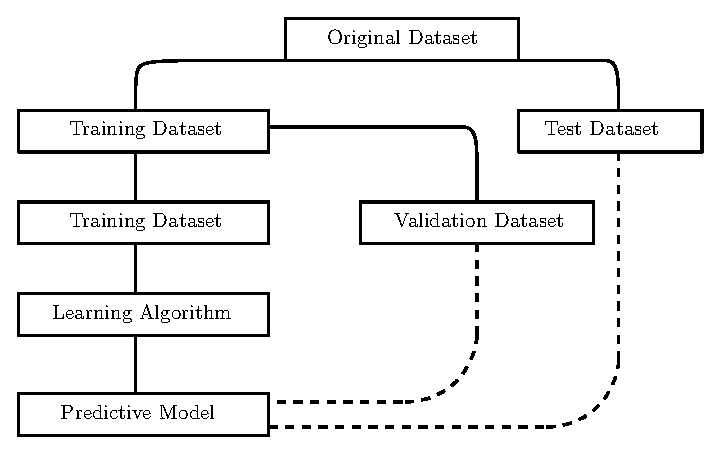
\includegraphics[width=.6\textwidth]{images/validation.eps}
%    \label{fig:cv}
%\end{figure}


%Figure \ref{fig:cv} presents a flowchart explaining how Cross Validation works. The same procedure was performed for the models estimated in this work (LASSO, Adaptive LASSO, and Elastic Net). Both the training, validation, and test dataset division were done randomly using the texttt{Matrix} \cite[]{matrix2020cran} package of the R software.\\


\section{Procedure and Cross Validation} \label{sec:cv}

In terms of organizational and methodological structure of the work, lexicons are used in the initial process in order to process the texts as a whole and extract the index of feelings.\\

As an initial procedure, the first necessary methodology input is the ECB speeches. A textual corpus is created from the discourses -- a corpus can be defined as a database that contains a set of texts, each with its respective Id for organizational purposes. In this work, the corpus used has, in addition to Id and texts, a column of dates, referring to the temporal moment of each discourse. With this database, a lexicon reading algorithm is applied to the texts and the referring feelings are extracted when in relation to the VADER and LM-SA-2020 lexicons in order to obtain the referring values for the sentiment variables.\\

The other necessary methodological input refers to the economic variables: from the dataset obtained from the corpus, it is necessary to merge these data with the economic variables in order to obtain, again, a new dataset. The last step in the data manipulation and organization process is data wrangling -- data wrangling is the process of altering and mapping data to make it more suitable and valuable for various downstream applications such as analytics \cite[]{dplyr2022, wickham2016r}. In this part of the process, operations to treat missing values and outliers were used, so that the obtained database is ``clean'' and usable for statistical and econometric modeling.\\

Finally, the last part of the methodological process is the part referring to econometric modeling and the so-called Cross Validation procedure. Cross Validation is a technique widely described in the literature \cite[]{hoornweg2018science, hastie2009elements, stone1974cross, breiman1992submodel} that aims to obtain optimal parameters from a predefined model. In Cross Validation, the dataset is divided between a training dataset and a test dataset, these being composed of 80\% and 20\% of the original dataset \cite[291]{breiman1992submodel}. The model, then, ``is estimated with a training sample and these estimates are used to ‘predict’ the outcomes of the validation sample. By varying the choice of a tuning parameters, one can select the set of configurations that leads to the best pseudo-out-of-sample forecasts''\cite[p.136]{hoornweg2018science}.\\

That said, the same methodology was used. The organization of the work starts from two initial points: the collection of economic variables and the collection of speeches from the European Central Bank\footnote{see section \ref{sec:ref}, chapter \ref{cap:results}}. From the speeches, a corpus is obtained in which the speech Ids are organized into dates and two lexicons exposed here are applied: VADER and LM-SA-2020 -- the result is stored in the dataset that contains the variables economic. As a standard methodology, the dataset is divided into a training and a test set (with a proportion of 80\% for the training set and 20\% for the test set), and the VAR models and the LASSO models. It should be noted, however, that for the estimation of the LASSO models, the cross validation procedure was used to obtain the optimal parameters of $\alpha$ and $\lambda$ -- the training set is divided into a validation set and another test set. The models are then estimated according to a variation in the parameters of $\alpha$ and $\lambda$ and confronted with the validation set, in order to verify the best model according to the metric evaluation criteria used. Figure \ref{fig:diagram} presents the organizational diagram of the project.\\

Four evaluation metrics criteria were taken into consideration when performing the cross validation procedure for the variable selection models. The $R^2$ \cite{heinisch1962steel}, the MAE \cite{willmott2005advantages}, the MSE \cite{bickel2015mathematical}, and the RMSE \cite{hyndman2006another}. Based on these criteria, the values of $\lambda$ were selected for the LASSO and Adaptive LASSO models, and the values of $\lambda$ and $\alpha$ for the Elastic Net model. For the VAR models, in addition to the AIC and BIC selection criteria, the Hannan–Quinn information criterion \cite{hannan1979determination} was also used to choose the best order of the model.\\



\begin{landscape} % CORRIGIR TRAINING
\begin{figure}
    \centering
    \caption{Diagram of the Methodology Used}
    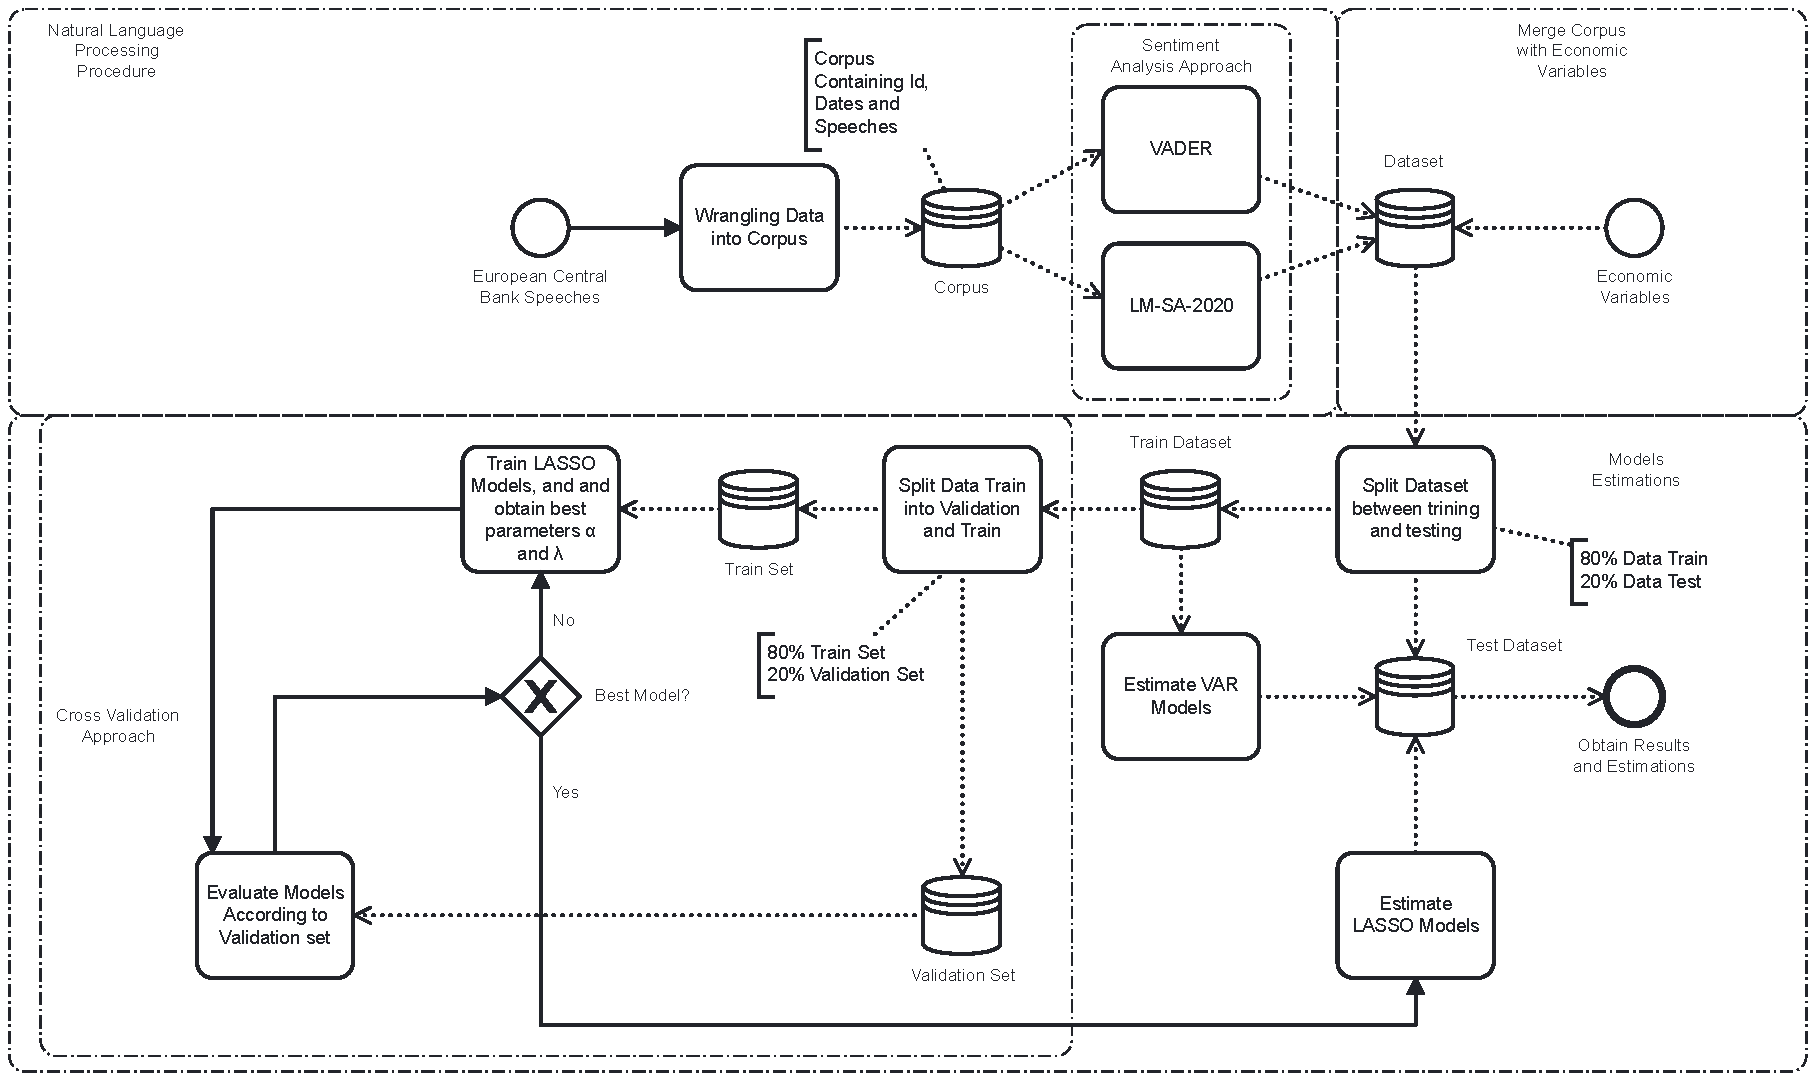
\includegraphics[width = \linewidth]{images/diagram2.pdf}
    \caption*{Note: the procedure described in the flowchart defines the evolution of the project in order to describe the general procedures used. For information about the databases used, the \href{https://github.com/gustavovital/Dissertation/tree/main/data}{database repository} is free to consult.}
    \label{fig:diagram}
\end{figure}
\end{landscape}






